% This is a LaTeX Template for course assignment designed by Hao Yin on March 9th, 2015.
% If you want to modify this template, go to Library  -->  Texshop  -->  Template  -->  ...

\documentclass[11pt, oneside]{article}      % use "amsart" instead of "article" for AMSLaTeX format
%\usepackage{geometry}                      % See geometry.pdf to learn the layout options. There are lots.
\usepackage[text={7in,9in},centering]{geometry}
\geometry{letterpaper}                          % ... or a4paper or a5paper or ...
%\geometry{landscape}                       % Activate for for rotated page geometry
%\usepackage[parfill]{parskip}          % Activate to begin paragraphs with an empty line rather than an indent

\usepackage{amsmath, amssymb, color}
%\usepackage{amsthm}
\usepackage{hyperref, url}
\usepackage{graphicx}               % Use pdf, png, jpg, or eps§ with pdflatex; use eps in DVI mode. TeX will automatically convert eps --> pdf in pdflatex



\usepackage{natbib} % This part is for bibliography.
 \bibpunct[, ]{(}{)}{,}{a}{}{,}%
 \def\bibfont{\small}%
 \def\bibsep{\smallskipamount}%
 \def\bibhang{24pt}%
 \def\newblock{\ }%
 \def\BIBand{and}%

% New environment part
\newtheorem{definition}{Definition}
\newtheorem{assumption}{Assumption}
\newtheorem{fact}{Fact}
\newtheorem{theorem}{Theorem}%[section]
\newtheorem{lemma}[theorem]{Lemma}
\newtheorem{corollary}[theorem]{Corollary}
\newtheorem{proposition}[theorem]{Proposition}
\newtheorem{claim}[theorem]{Claim}
\newtheorem{remark}{Remark}
\newtheorem{example}{Example}
% Need the environment Proof ? Please use the following:
% {\noindent\bf Proof.}  ...........................  $\hfill \square$\\

% Bold type part.
\newcommand{\ba}{\mbox{\boldmath $a$}}
\newcommand{\bb}{\mbox{\boldmath $b$}}
\newcommand{\bc}{\mbox{\boldmath $c$}}
\newcommand{\bd}{\mbox{\boldmath $d$}}
\newcommand{\be}{\mbox{\boldmath $e$}}
\newcommand{\bff}{\mbox{\boldmath $f$}} %NOTICE!
\newcommand{\bg}{\mbox{\boldmath $g$}}
\newcommand{\bh}{\mbox{\boldmath $h$}}
\newcommand{\bo}{\mbox{\boldmath $o$}}
\newcommand{\bp}{\mbox{\boldmath $p$}}
\newcommand{\bq}{\mbox{\boldmath $q$}}
\newcommand{\br}{\mbox{\boldmath $r$}}
\newcommand{\bs}{\mbox{\boldmath $s$}}
\newcommand{\bt}{\mbox{\boldmath $t$}}
\newcommand{\bu}{\mbox{\boldmath $u$}}
\newcommand{\bv}{\mbox{\boldmath $v$}}
\newcommand{\bw}{\mbox{\boldmath $w$}}
\newcommand{\bx}{\mbox{\boldmath $x$}}
\newcommand{\by}{\mbox{\boldmath $y$}}
\newcommand{\bz}{\mbox{\boldmath $z$}}
\newcommand{\bzero}{\mbox
%{\Large 
{\boldmath $0$}}
%}

\newcommand{\bA}{\mbox{\boldmath $A$}}
\newcommand{\bB}{\mbox{\boldmath $B$}}
\newcommand{\bC}{\mbox{\boldmath $C$}}
\newcommand{\bD}{\mbox{\boldmath $D$}}
\newcommand{\bI}{\mbox{\boldmath $I$}}
\newcommand{\bM}{\mbox{\boldmath $M$}}
\newcommand{\bU}{\mbox{\boldmath $U$}}
\newcommand{\bV}{\mbox{\boldmath $V$}}
\newcommand{\bW}{\mbox{\boldmath $W$}}
\newcommand{\bX}{\mbox{\boldmath $X$}}
\newcommand{\bY}{\mbox{\boldmath $Y$}}
\newcommand{\bZ}{\mbox{\boldmath $Z$}}

\newcommand{\balpha}{\mbox{\boldmath $\alpha$}}
\newcommand{\bbeta}{\mbox{\boldmath $\beta$}}
\newcommand{\btheta}{\mbox{\boldmath $\theta$}}
\newcommand{\bgamma}{\mbox{\boldmath $\gamma$}}
\newcommand{\bdelta}{\mbox{\boldmath $\delta$}}
\newcommand{\bmu}{\mbox{\boldmath $\mu$}}
\newcommand{\bepsilon}{\mbox{\boldmath $\epsilon$}}
\newcommand{\blambda}{\mbox{\boldmath $\lambda$}}
\newcommand{\btau}{\mbox{\boldmath $\tau$}}
\newcommand{\bsigma}{\mbox{\boldmath $\sigma$}}
\newcommand{\bSigma}{\mbox{\boldmath $\Sigma$}}

% Specific math notation:
\newcommand{\real}[1]{\mbox{$\mathbb{R}^{#1}$}}
\newcommand{\prob}{\mbox{$\mathbb{P}$}}
\newcommand{\expect}{\mbox{$\mathbb{E}$}}
\newcommand{\var}{\mbox{$\mathbb{V}$}}
\newcommand{\compl}[1]{\mbox{$\mathbb{C}^{#1}$}}
\newcommand{\realN}[1]{\mbox{$\real{I_1 \times I_2 \times \dots \times I_{#1}}$}}
\newcommand{\complN}[1]{\mbox{$\compl{I_1 \times I_2 \times \dots \times I_{#1}}$}}
%\newcommand{\natural}{\mbox{$\mathbb{N}$}}

% Enumerate part
\newcommand{\V}[1]{\mbox{\boldmath $#1$}}
\newcommand{\RV}[1]{\mbox{\boldmath $\tilde{#1}$}}
\newcommand{\rv}[1]{\tilde{#1}}
\newcommand{\OPT}{{\mbox{OPT}}}
\newcommand{\SP}{{\tt{SP}}}
\newcommand{\CVX}{{\tt{CVX}}}
\newcommand{\LP}{{\tt{LP}}}
\newcommand{\D}{{\tt{D}}}
\newcommand{\ALG}{\tt{ALG}}
\newcommand{\cT}{{\cal T}}

%Added on Feb 23, 2015: Roman numbers, chapters, DEFINE format
\newcommand{\rmnum}[1]{\romannumeral #1} % Roman small letter
\newcommand{\Rmnum}[1]{\uppercase\expandafter{\romannumeral #1}} % Roman capital letter
\usepackage[raggedright]{titlesec}% 可换为 raggedleft  raggedright
\titleformat{\chapter}{\centering\Huge\bfseries}{Chapter \Rmnum{\thechapter} }{1em}{} % in book format
\newcommand{\df}{\bfseries \em}  % DEFINE format for text

%Added on April 30th, 2015: 
\usepackage{mathrsfs} %math-script format, then use \mathscr{F} 
\usepackage{enumerate} % change the symbols in enumerate
\graphicspath{{figures/}}  %图片路径

%Added on Jul 11th, 2015:
\newcommand{\tensorA}{\mbox{\boldmath $\mathcal{A}$}}
\newcommand{\tensorD}{\mbox{\boldmath $\mathcal{D}$}}
\newcommand{\tensorE}{\mbox{\boldmath $\mathcal{E}$}}
\newcommand{\tensorF}{\mbox{\boldmath $\mathcal{F}$}}
\newcommand{\tensorG}{\mbox{\boldmath $\mathcal{G}$}}
\newcommand{\tensorI}{\mbox{\boldmath $\mathcal{I}$}}
\newcommand{\tensorU}{\mbox{\boldmath $\mathcal{U}$}}
\newcommand{\tensorV}{\mbox{\boldmath $\mathcal{V}$}}
\newcommand{\tensorX}{\mbox{\boldmath $\mathcal{X}$}}
\newcommand{\tensorY}{\mbox{\boldmath $\mathcal{Y}$}}
\usepackage{multirow}
\usepackage{amsmath} 
\usepackage{stmaryrd}
\usepackage{float}
\usepackage{graphicx}
\usepackage{subfigure}
\usepackage{xcolor} 
\DeclareMathOperator*{\argmin}{argmin}

\usepackage{color}
\newcommand{\tbw}{\bigskip \mbox{\color{red} {\df (TBW) }}\bigskip}

%\newcommand{\hasPageBreak}{\newpage}
\newcommand{\hasPageBreak}{}


% Added on Dec 8th, 2015: listings
\usepackage{listings}

% Added on March 9th, 2016: algorithm
\usepackage{algorithm} 
\usepackage{algorithmic}
\renewcommand{\algorithmicrequire}{\textbf{Input:}}
\renewcommand{\algorithmicensure}{\textbf{Output:}}

\begin{document}
\title{Answer to CS224n Assignment 3}
\author{
Pengfei Gao, Fanny Yang, Hao Yin 
\thanks{\texttt{\{pfgao, fanfyang, yinh\}@stanford.edu}. 
Each member contributes equally, and names are put in alphabetic order.} 
}
\date{}
\maketitle

\section*{Problem 1}
\begin{enumerate}   [(a)]
%\setcounter{enumi}{3}
\item 
\begin{enumerate}   [i]
%\setcounter{enumi}{3}
\item 
Stanford just offered me a big fellowship. [Stanford here may mean an ORG (Stanford university) or a PER]

Go Giant! [Giant may mean an ORG(SF Giant) or a PER (named Giant) or null (a huge creature)]

\item
We may need context as an important information in inferring NER. For example, if you say George Stanford is a great man, then Stanford is a PER; if you say Stanford University, then Stanford is an ORG.

\item 
The proceeding word of the target, e.g., if the proceeding word is `a`, `the' or `at', `in'.

The first letter of that word is capital or not.

\end{enumerate}


\hasPageBreak
\item
\begin{enumerate}   [i]
%\setcounter{enumi}{3}
\item 
$\be \in \real{1 \times (2 w + 1) D}$, $W \in \real{(2 w + 1)D \times H}$, $U \in \real{H \times C}$.


\item For each time step, forming $\be$ takes $O((2 w + 1) D)$, computing $\bh$ takes $O((2 w + 1)DH)$, then computing $\hat \by$ takes $O(HC)$. Therefore, for each time step, the total time for predicting label complexity is $O(H((2 w + 1)D + C))$. Now for a sentence of length $T$, the total time complexity is 
\[O(HT((2 w + 1)D + C)).\]

\end{enumerate}




\item
See my code submission as well as \texttt{window\_predictions.conll}.



\hasPageBreak
\item
\begin{enumerate}   [i]
%\setcounter{enumi}{3}
\item 
The best development entity-level $F_1$ score is 0.84, and the corresponding confusion matrix is:

\begin{figure}[htbp] %  figure placement: here, top, bottom, or page
   \centering
   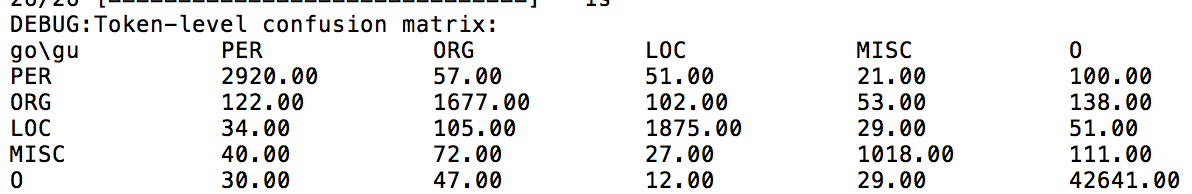
\includegraphics[width=5.2in]{Q1_confusion.png} 
   \caption{Token-level confusion matrix}
   \label{Fig:Q1_confusion}
\end{figure}

According to the confusion matrix, it is easy to mistakenly predict a PER as a ORG, predict ORG as LOC, and predict LOC as ORG.


\item
One limitation is the prediction of the current word is not related with the prediction of the proceeding word (only related with the representation of the proceeding word). This will make mistakes like the following:

\begin{figure}[htbp] %  figure placement: here, top, bottom, or page
   \centering
   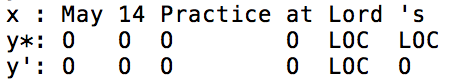
\includegraphics[width=3.2in]{Q1_error1.png} 
   \caption{Error1}
   \label{Fig:Q1_error1}
\end{figure}

where it predict 's to O while the true label LOC follows from the label of the proceeding word ``Lord", which is LOC.


Another limitation is window size can only be limited, i.e., one can only handle windows of moderate size, not of arbitrary length. By fixing a small size of window, one might loose some important context. Example is the following:
\begin{figure}[htbp] %  figure placement: here, top, bottom, or page
   \centering
   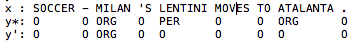
\includegraphics[width=3.2in]{Q1_error2.png} 
   \caption{Error2}
   \label{Fig:Q1_error2}
\end{figure}

In predicting LENTINI, window of size 1 can only see 'S and MOVES, but the most important context in this sentence is SOCCER (from which we will know that LENTINI is the soccer player)



\end{enumerate}



\end{enumerate}







\hasPageBreak
\section*{Problem 2}
\begin{enumerate}   [(a)]

\item 
\begin{enumerate}   [i]
\item $W_h \in \real{H \times H}$, 
		$W_x \in \real{D \times H}$, 
		$\bb_1 \in \real{H}$, 
		$U \in \real{H \times C}$, 
		$\bb_2 \in \real{C}$
There are $H^2+DH+H+HC+C$ parameters for RNN.
Compared to $(2w+1)D+(2w+1)DH+HC$ parameters for forward NN.
\item To calculate next state cost $O(H(H+D))$.Calculate softmax cost $O(HC)$. Therefore, total cost is $O(HT(H+D)+HC)$.
\end{enumerate}

\item
\begin{enumerate}   [i]
\item Since cross-entropy loss only has a effect on the true label's negative log-likelihood. For a single sample, the cross-entropy loss is equal to the negative log-likelihood of classifying it to be true label. The loss property is decreasing with a smaller and smaller gradient as p goes up. Suppose we have 99 correctly predicted samples of which the probability of classifying true label is 0.5001; 1 incorrectly predicted sample of which the probability of classifying correct label is 0.0001. If we tune our model parameter, we could make the incorrect sample to have a 0.4999 probability for true label while the 99 correct samples to have a 0.4999 probability as well. In this case, cross-entropy loss will drop tremendously but the F1 score actually drops to zero.
\item First, precision and recall are discontinuous measures, which cannot be optimized by gradient methods. Second, the harmonic mean makes it hard to calculate gradient.
\end{enumerate}
\item code
\item 
\begin{enumerate}   [i]
\item The loss and gradient after $t=T$ is uselessly added into total objective if there is no masking. Masking multiplies zero to these useless terms to make sure they have no effect.
\end{enumerate}

\item code
\item running code and report results
\item 
\begin{enumerate}   [i]
\item (This part needs observing the result first)  \\
 Limitation 1: \tbw \\
 Limitation 2: \tbw 
 \item Solution for 1: \tbw \\
 Solution for 2: \tbw
\end{enumerate}

\end{enumerate}




\hasPageBreak
\section*{Problem 3}
\begin{enumerate}   [(a)]
%\setcounter{enumi}{3}
\item 
\begin{enumerate}   [i]
%\setcounter{enumi}{3}
\item $w_h = 1$, $u_h = 1$, $b_h = 0$.
\item $w_z = 1$, $u_z = 0$, $u_h = 1$, and then $w_h$ can be any number.
\end{enumerate}






\hasPageBreak
\item
\begin{enumerate}   [i]
%\setcounter{enumi}{3}
\item 
We show that the parameter values that realizes this  behavior do not exist. 

Suppose $h^{(t-1)} = 0$, then $x^{(t)} = 1$ must lead to $h^{(t)} = 1$ while $x^{(t)} = 0$ must lead to $h^{(t)} = 0$, thus
\begin{eqnarray*}
u_h + b_h &>& 0,
\\
b_h &\leq& 0,
\end{eqnarray*}
from which we know that $u_h > 0$. Now suppose $h^{(t-1)} = 1$, then $x^{(t)} = 1$ must lead to $h^{(t)} = 0$ while $x^{(t)} = 0$ must lead to $h^{(t)} = 1$, thus
\begin{eqnarray*}
u_h + w_h + b_h &\leq& 0,
\\
w_h + b_h &>& 0,
\end{eqnarray*}
from which we know that $u_h < 0$. Therefore, we must have $u_h > 0$ and $u_h < 0$, which is a contradiction.



\item
$b_r = 1$, $w_z = 1$, $u_z = -1$, $w_h = -1$, $u_h = 1$.
\end{enumerate}


\item
See my code submission


\hasPageBreak
\item Learning curves are as below:

\begin{figure}[htbp] %  figure placement: here, top, bottom, or page
   \centering
\begin{minipage}{0.5\linewidth}\centering
   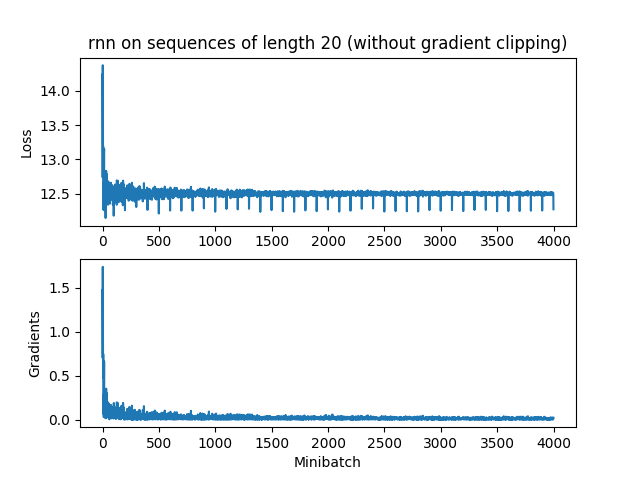
\includegraphics[width=3.8in]{q3-noclip-rnn.png} 
   \\{\footnotesize  RNN without clip  }
\end{minipage}
\begin{minipage}{0.49\linewidth}\centering
   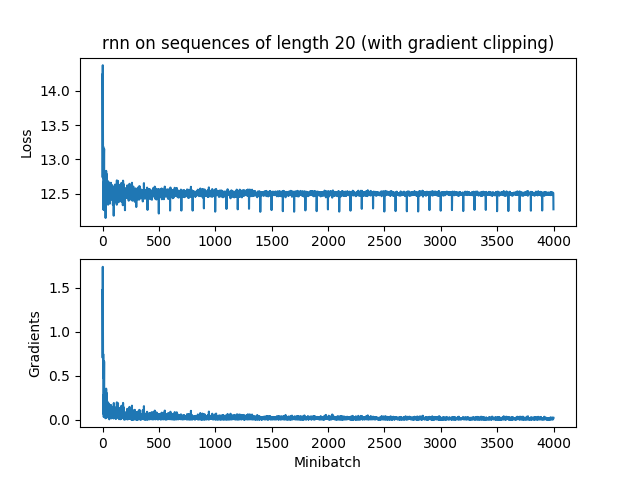
\includegraphics[width=3.8in]{q3-clip-rnn.png} 
   \\{\footnotesize  RNN with clip  }
\end{minipage}
\begin{minipage}{0.5\linewidth}\centering
   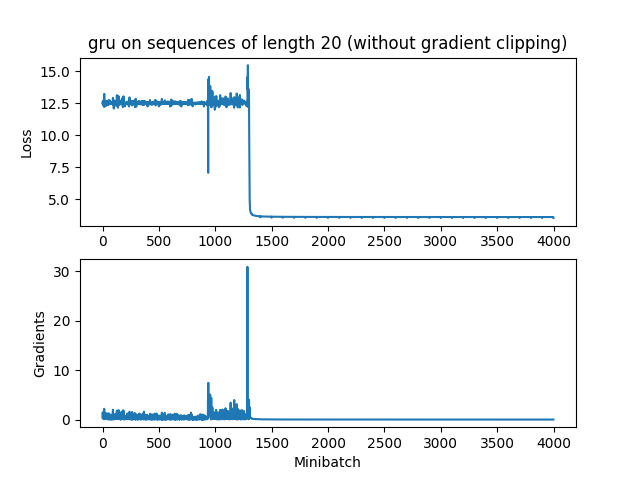
\includegraphics[width=3.8in]{q3-noclip-gru.png} 
   \\{\footnotesize  GRU without clip  }
\end{minipage}
\begin{minipage}{0.49\linewidth}\centering
   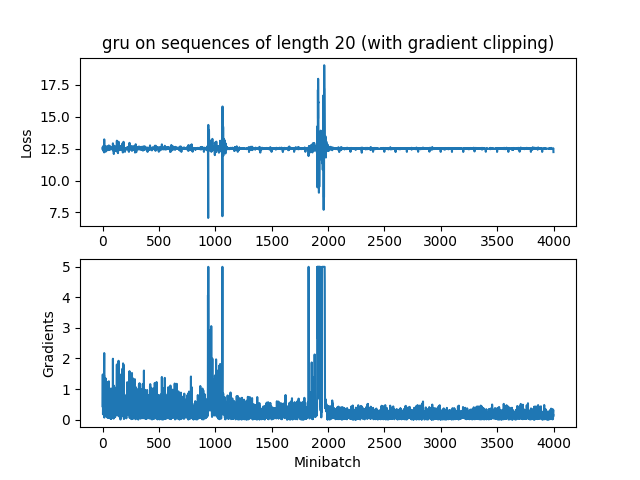
\includegraphics[width=3.8in]{q3-clip-gru.png} 
   \\{\footnotesize  GRU with clip  }
\end{minipage}
\caption{Learning curves}
\label{Fig:Q3d}
\end{figure}

\hasPageBreak
\item
\begin{enumerate}  [i]
%\setcounter{enumi}{3}
\item 
RNN experiences vanishing gradients, and neither model experience exploding gradients. 
The gradient clipping does not help.


\item The GRU model works better. The reason is that GRU model does not experience vanishing gradient, thus any word in the sentence can provide information in back-propagation (parameter training).


\end{enumerate}


\item See code submission as well as \texttt{window\_predictions.conll}. 
\end{enumerate}





\bibliographystyle{ormsv080}  % Need the file `` ormsv080.bst '' at the same folder.
\bibliography{Bibli}  % Need the file ``Bibli.bib '' in the same folder.
\end{document}